\chapter{Missing epidemiological parameter data: traumatic brain injury}
\label{applications-double_dismod}

TK intro about double dismod, to deal with acute and chronic phase of disease.
TK is the focus of this chapter estimating prevalence using incidence data
or using splitting the disease into short and long term illnesses?

The compartmental model assumes a constant mortality hazard.
However, traumatic brain injury (TBI) has a wide range of
causes, ranging from unintentional falls to traffic injuries.
Given some cases suffer acute injury while others sustain
chronic conditions, the burden of the disease and the mortality hazard
differ by cause.  Hence the compartmental model must be modified
to avoid violating the model assumption of a
constant mortality hazard.  To address this disparity in mortality
risk, TBI can be divided into short term and long term
causes.  This method is also necessary for other injuries and
diseases such as heart attack and stroke.

For whatever reason, data are often not available for one or more
epidemiological parameters.  In the GBD 2010 study, this is
problematic when the missing parameter is needed for the calculation
of disease burden.  Injuries provide an excellent example of missing
epidemiological parameter data as incidence is often only reported.

TBI is a major cause of morbidity and
mortality in young individuals. Commonly caused by traffic
incidents, falls, interpersonal violence or sports injuries,
TBI may result in physical, cognitive, and psychosocial impairment.
It is typically diagnosed by clinical symptoms such as loss of
consciousness or amnesia. \cite{maas_moderate_2008, nih_rehabilitation_1999,
bruns_epidemiology_2003}

Data only include cases warranting hospital care and cases warranting
treatment by health care professional but not hospitalization (other
health care).  As seen in Figure \ref{fig:app-injury brain fit},
only incidence data were available from hospital discharge records.

To estimate prevalence, incidence data are used in a compartmental model to estimate the
age-specific burden of TBI, as shown in Figure
\ref{fig:app-injury brain fit}.  By fitting all of the epidemiological
parameters together, the compartmental model can estimate prevalence
without prevalence data.  Without the compartmental model, TK another method.

Focusing solely on long term TBI, the compartmental model simultaneously fits all epidemiological parameters to estimate TBI
prevalence, as see in Figure \ref{fig:app-injury brain fit}.  TK better
description of what compartmental model did and how hard it would be any other way

    \begin{figure}[h]
        \begin{center}
            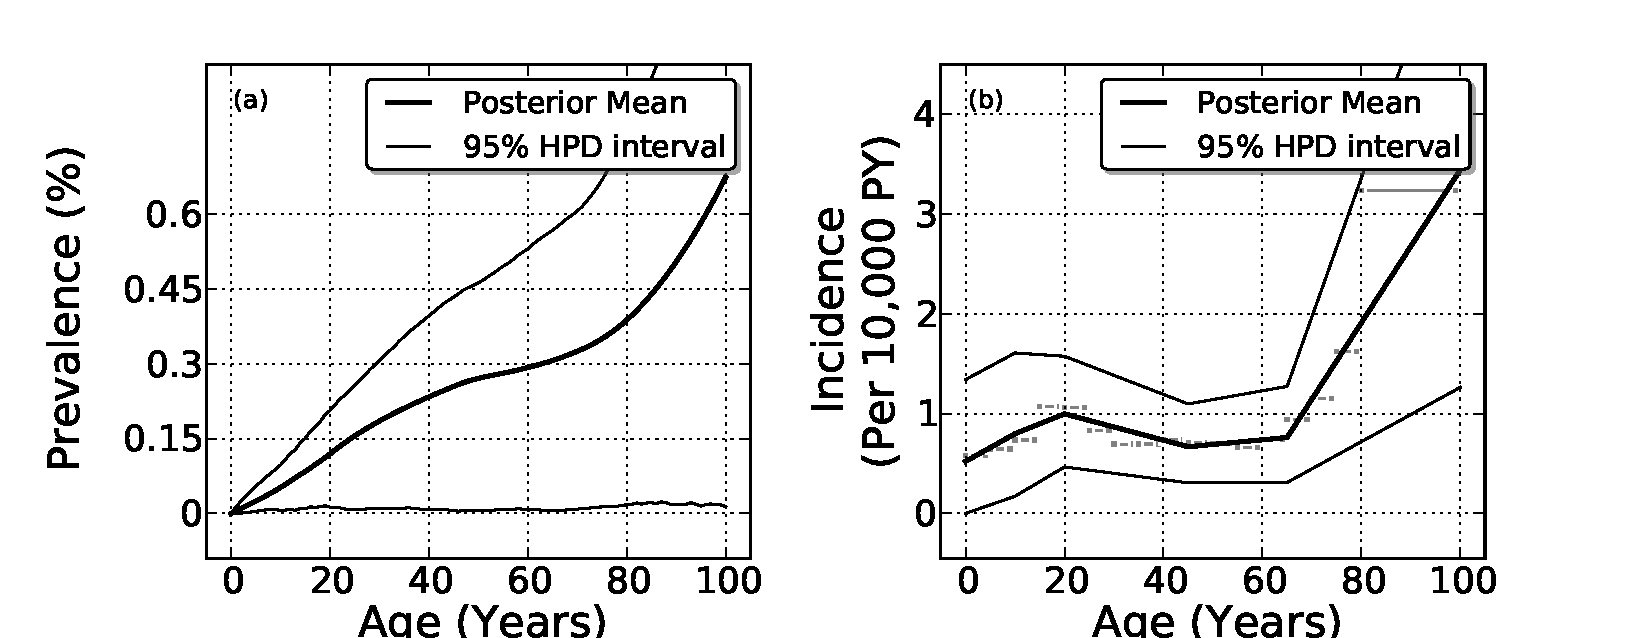
\includegraphics[width=\textwidth]{injuries-con_fit_p.pdf}
            \caption{Prevalence (a) and incidence (b)
              estimates for males in the United States of America in
              2005 with moderate to severe TBI.}
            \label{fig:app-injury brain fit}
        \end{center}
    \end{figure}

TK conclusion about compartmental model saving the day

